\chapter{时间信息增强的视频目标跟踪算法研究}\label{chap:end}
在上一章中,我们研究了如何为基于孪生网络的视频目标跟踪算法提供更丰富的空间信息以克服跟踪的累计误差。然而,如何在基于孪生网络的视频目标跟踪算法中利用\textbf{时间信息}尚未得到广泛研究。在本章中,我们提出了一种新型孪生跟踪体系结构,配备有一个时间聚合模块,该模块通过聚合来自相邻帧的时间信息来改善每帧的特征。这种时间聚合策略使孪生跟踪器可以处理由于运动模糊等原因导致的目标表观信息退化现象。此外,我们在孪生网络中整合了对抗性 Dropout 模块,以端到端的方式学习更具判别性的目标特征。本章通过在 GOT-10k \cite{GOT-10k} 和 UAV20L \cite{mueller2016benchmark} 数据集上的大量实验结果,证明了基于时间信息增强的跟踪系统的有效性。

\section{引言}
\label{sec:intro}
视频目标跟踪的目的是在视频序列每一帧中估计任意目标的状态。 
最近,孪生网络已经为目标跟踪的性能带来显著提高。然而,由于视频中由于运动模糊等原因导致的目标表观信息退化(图\ref{fig:visulization}),往往造成学习到的通用特征表示的判别力下降。
研究人员尝试了不同的方法来改进特征表示。
例如,
%RASNet \cite{wang2018learning} explores diverse attention mechanisms to adapt the offline learned feature representations to a specific tracking target.
SA-Siam \cite{he2018twofold} 分别训练两个分支,以保持语义特征和表观特征的异构性。
在 DaSiamRPN~\cite{zhu2018distractor} 中,作者设计了一个可感知近似物体的增量学习模块,该模块可以有效地将通用嵌入特征迁移到当前视频域,并在推理过程中增量捕获目标表观变化。
SiamRPN++~\cite{SiamRPN++} 引入了一种简单而有效的采样策略,以更强大的深度架构来驱动孪生跟踪器。
上述方法从不同的角度改善了目标的特征表示,并提高了视频目标跟踪算法的性能。
%These improvements are useful.
%However, all these effort ignores a important problem: they ignore to merge the inter-frame feature during the training phase.
%One important solution is use the temporal information.
%The use of temporal information is important because, when one frame is bad, the adjusting frame can be used. While several method trying to use the temporal information, the method is naive.
%(The bug is, I cannot find any temporal information used in siamese trackers. (I cannot believe it!!! Check it again.--Checked)) For example, A use a time memory to store the appearance information. B use a simple feature average during test. C use history positional information to predict the object position in current frame. However, all these method cannot handle the temporal information during training, which lead to sub-optimal result. To solve this problem, 
然而,这些方法仅利用从当前帧裁剪的特征执行跟踪,这限制了孪生跟踪器的性能。

实际上,视频具有关于目标的丰富信息,并且这种时间信息是视频理解和跟踪的重要基础。
例如,在视频目标检测中,FGFA~\cite{zhu2017flow} 在特征级别上利用了时间一致性。该算法通过沿运动路径聚聚合相邻的特征来改善每帧特征,从而提高了视频识别精度。
在视频目标分割中,STCNN~\cite{xu2019spatiotemporal} 引入了时间模块,该模块着重于捕获动态表观和运动线索以提供目标分割的指导信息。
在基于判别性相关滤波器的目标跟踪中,FlowTrack~\cite{zhu2018end} 专注于利用连续帧中丰富的流信息来改善特征表示和跟踪精度。
但是,如何在孪生跟踪器中利用时间信息尚未得到广泛研究。

\begin{figure*}[t]
    \centering
    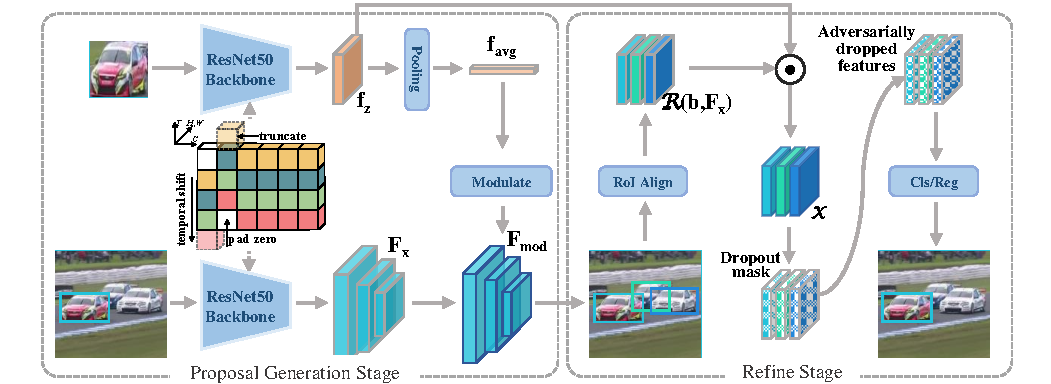
\includegraphics[width=1.0\textwidth]{Img/end/net_v3.pdf}
    \caption{
    本章提出的两阶段 SiamTFA 概述。
    %At the first stage, a siamese FPN equipped with a temporal aggregation module provides features of the template image and the search image. Then the feature modulation module is used to merge the features and generate proposals.
    %proposals of the object given in the first-frame bounding box. 
    %At the second stage, 
    候选生成阶段旨在生成视觉表观上类似于给定模板目标的候选目标区域。细化阶段旨在从候选目标区域中选择目标。}
    \label{fig:SiamTFA}
\end{figure*}

% key words: temporal modeling, model the temporal information, temporal fusion, inter-frame information, improve the feature representation, temporal aggregation, poor object appearance
在本章中,我们旨在充分利用孪生跟踪器中的时间信息。
%(We introduce a novel siamese tracking architecture equipped with a temporal aggregation module to make full use of inter-frame information.)
%(In this work, to deal with the issues raised above, we propose a novel tracker to aggregate features of adjacent frames by ...)
%(In this paper, we develop an end-to-end temporal aggregation module in siamese architecture to utilize both the power of siamese trackers and the inter-frame information.)
我们提出了一种新型孪生跟踪体系结构,配备有时间聚合模块,该模块通过聚合相邻帧中的特征来改善每帧中目标的特征表示。
这种时间聚合策略使孪生跟踪器可以处理由于运动模糊等原因导致的目标表观信息退化现象。
为实现聚合时间信息的目的,我们在孪生网络的特征提取网络中沿时间维度 \cite{lin2019tsm} 移动通道特征。
请注意,由于视频中目标的运动 \cite{zhu2017flow},相邻帧中同一目标的特征通常不会在空间上对齐,因此仅对残差层 \cite{lin2019tsm} 进行时间平移,以保证孪生跟踪器的特征学习能力。
与其他时间融合方法 \cite{tao2016siamese, gladh2016deep} 不同,本章采用的方法能够在大规模数据集上进行端到端的训练。
%本章提出的时间聚合模块在孪生网络中进行了端到端的培训。
%The proposed temporal aggregation module is trained end-to-end in the siamese network.
%(This module enables our module to be trained end-to-end on large-scale datasets.)
此外,本章采用的时间融合方法易于实现,而无需更改孪生跟踪架构或使用光流 \cite{zhu2018end} 信息。

%improve the generalization ability on bad object.
%Our insight is that, if we only rely on the traditional training method, the bad image in the training data will be over wheeled by the easy cases. So the tracker shows bad performance when meeting with bad image during testing. To solve this problem, we take advantage of the recent progress in adversarial learning to increase the robustness of object features.
%Our method employs adversarial Dropout to increase the robustness of object features. 
%注意,由于该模块在文章中占据次要位置,所以不应该写目前方法存在的缺点,而应该直接写用了这个模块后起到的作用。
%感觉概括性的优点不太好想,所以可以多些几句实现细节。这就要求我们弄懂代码原理。
为了提高目标特征的鲁棒性,我们在孪生跟踪网络中进一步整合了一个对抗性 Dropout \cite{park2018adversarial} 模块。
% add adversarial Dropout to enforce the tracker to learn difficult cases. 
% (We further propose a adversarial training module to enforce the tracker to learn difficult cases. The motivation is that ... This is achieved by computing the adversarial masks based on diversity maximum. This simple form of feature selection improves the discrimination power of the tracker.)
%Specifically, we calculate the diversity of two Dropouts, and make the loss max to learn the difficult Dropout mask.
具体而言,首先根据散度最大值预测对抗性 Dropout 模板。
然后,我们旨在最大程度地减小随机删除的特征和对抗删除的特征之间的差异。
%The effect of this module can be interpreted from both the Dropout and from the adversarial training perspectives.
该模块具有 Dropout 和对抗训练的双重优势:Dropout 使基于孪生网络的视频目标跟踪器在训练过程中随机断开神经元,以防止目标特征的过拟合;而对抗训练则使基于孪生网络的视频目标跟踪器学习困难的情况。

总体来说,本章的贡献有三个方面:
\begin{itemize}
\item 在本章中,我们提出了一种新型孪生跟踪体系结构,配备有时间聚合模块,可通过聚合相邻帧的特征来改善每帧中目标的特征表示。
\item 我们在孪生网络跟踪器中进一步引入了对抗性 Dropout 模块,以提高孪生跟踪网络的特征判别能力。
\item 在 GOT-10k \cite{GOT-10k} 和 UAV20L \cite{mueller2016benchmark} 跟踪数据集上的大量实验结果,证明了基于时间信息增强的跟踪系统的有效性。(图 \ref{fig:visulization})。
\end{itemize}

\section{相关工作}
\subsection{时间信息在视频动作识别中的应用}
远程时间结构在理解动作视频的动态过程中起着重要的作用。但是,主流的卷积神经网络框架通常集中在表观信息和短期运动上,因此缺乏整合远程时间结构的能力。最近,有一些尝试 \cite{Motionlets} 来解决这个问题。这些方法主要依赖于具有预定采样间隔的密集时间采样。当将这种方法应用于长视频序列时,将导致过高的计算成本,这限制了其在现实世界中的应用,并存在丢失长视频中重要信息的风险。因此,在 \cite{TSN} 中,基于远程时态结构建模的思想,提出了一种视频动作识别的新型框架。该框架结合了稀疏的时间采样策略和视频级别的监督,可以使用整个动作视频进行高效地学习。该框架采用稀疏采样方案在长视频序列上提取短视频片段,其中采样点沿时间维度均匀分布。在此基础上,采用分层结构聚合来自采样视频段的信息。因此,该算法能够对整个视频的远程时间结构进行建模。此外,这种稀疏的采样策略可以使用较低的成本保存视频信息,从而可以在合理的时间和计算资源预算下,在长视频序列上进行端到端学习。% Temporal Segment Networks: Towards Good Practices for Deep Action Recognition 1608
在 \cite{TRN} 中,作者认为时间关系推理使人类能够根据过去情况分析当前情况,并就下一步可能发生的情况提出假设。时间关系推理对于视频动作识别至关重要,它构成了描述事件的基础。因此,作者提出了一种有效且可解释的网络模块,即时间关系网络(temporal relational reasoning,TRN),该模块旨在学习和推理多个时间尺度上视频帧之间的时间依赖性。% Temporal Relational Reasoning in Videos 1711
在 \cite{AdaFuse} 中,作者认为时间建模是有效的视频动作识别的关键。虽然了解时间信息可以提高动态动作的识别精度,但是消除时间冗余和重用过去的特征可以大大节省计算量,从而实现有效的动作识别。因此,作者提出了一种称为 AdaFuse 的自适应时间融合网络,该网络可以动态融合当前和过去特征图中的通道,以实现强大的时间建模,从而提高识别精度和效率。% ADAFUSE: ADAPTIVE TEMPORAL FUSION NETWORK FOR EFFICIENT ACTION RECOGNITION
\subsection{时间信息在视频目标检测中的应用}
在视频目标检测算法 TCNN \cite{TCNN} 中,作者认为在相邻帧中目标的位置和表观应保持连续性,即,预测的边界框位置和检测置信度不应在短时间内发生剧烈变化。然而,如果将图像目标检测框架直接应用于视频目标检测任务中,则目标的检测置信度往往会在相邻帧之间发生显著变化。为了解决这一问题,作者提出了一个深度学习框架,该框架扩展了流行的图像检测框架 R-CNN \cite{girshick2014rich} 和 Faster R-CNN \cite{ren2015faster},以通过合并相邻帧的时间信息和上下文信息来解决视频中的通用目标检测问题。该算法可以在相邻帧中传播检测结果,并可沿着跟踪算法生成的轨迹修改检测置信度,从而有效地提高现有图像检测框架的在视频目标检测任务中的性能。% T-CNN: Tubelets with Convolutional Neural Networks for Object Detection from Videos 1604
该工作虽然提高了识别准确性,具有较高的计算成本。为了减少计算量,在文献 \cite{DeepFeature} 中,作者了深度特征流,一种快速、准确的视频目标检测方法。该方法在稀疏的关键帧上应用图像检测网络,通过流场将深度特征图从关键帧传播到其他帧。传播后的特征类似于原始特征。通常,流估计和特征传播比卷积特征的计算快得多。因此,该方法避免了计算瓶颈,显著提高了检测速度。当流场也由网络估算时,整个架构将进行端到端训练,可同时优化目标检测任务和流网络。% Deep Feature Flow for Video Recognition
\subsection{时间信息在视频目标跟踪中的应用}
大多数现有的相关滤波跟踪器仅考虑当前帧的表观特征,几乎无法从运动和帧间信息中受益。在诸如部分遮挡和形变之类的挑战中,缺少时间信息会降低跟踪性能。目标跟踪所处理的是视频信息,因此时序信息很重要。以前有很多工作利用时序信息进行目标跟踪。
在文献 \cite{DeepMotion} 中,作者首次提出将表观信息与深度运动特征融合以进行视觉跟踪。表观特征仅对单帧中的静态信息进行编码,而深度运动特征则对基于光流的多帧信息进行整合。因此,运动特征可以捕获与表观特征互补的场景动态特征。因此,作者研究了深度运动功能对视频目标跟踪的影响,并提出将表观特征与深度运动特征进行融合,以进行视频目标跟踪。
该方法虽然利用光流提高了视频目标跟踪算法的性能,但采用的是在在动作识别任务中预训练的深层光流网络,并没有在视频目标跟踪任务中进行端到端训练,因此没有获得最佳跟踪效果。
为了解决这一问题,FlowTrack \cite{FlowTrack} 首次提出深度学习框架中共同训练光流网络和跟踪网络你,从而利用连续帧中丰富的光流信息进一步提高特征表示和跟踪精度。首先,作者将包括光流估计、特征提取、特征聚合和相关滤波器跟踪在内的各个组件制定为网络中的特殊层。然后,按照光流的引导,以指定的时间间隔对历史特征图进行扭曲并与当前特征图进行聚合,从而捕获视频中的时间信息。

\section{孪生网络跟踪器的端到端时间聚合}
\label{sec:method}
%应该提及我们的跟踪器的损失函数包括:对抗性损失,加上常规跟踪损失。
%In this section, we will introduce the proposed tracking method, SiamTFA (Fig. \ref{fig:SiamTFA}). 
%The main feature is:
%(1) A strong backbone. Use FPN and new-proposed feature modulation.
%(2) Equipped with 2 useful module: temporal aggregation module and adversarial Dropout module to improve the robustness of features.
%In the following, three sub-section will be introduced: (1) Overview of tracking (2) Temporal aggregation module (3) Adversarial Dropout module.
%网络结构怎么描述?可以参考ATOM。
%Our SiamTFA bases on a strong feature extractor -- FPN.
%We insert our temporal aggregation module in the backbone. Details of this module will be introduced at sec 3.2.
%Be robust to object size.
%FPN: handle different object size.
%modulator vector: handle different template object size.
%xcorr depth-wise: stage1 merge.
%element wise product: stage2 merge
% 介绍输入
%The input of the network is ... We use notations ... to denote ..., respectively. ... has a size of ...
%SiamTFA is composed of ... and ...
%Inspired by the great success of siamese trackers \cite{SiamRPN++, Wang2018SiamMask}, we also construct our SiamTFA based on the siamese architecture.
在本节中,我们将介绍基于孪生体系结构的跟踪方法,即 SiamTFA(图 \ref{fig:SiamTFA}),其灵感来自孪生跟踪器 \cite{SiamRPN++, Wang2018SiamMask} 的巨大成功。
具体而言,SiamTFA 将图像对作为输入,包括模板图像和搜索图像。模板图像是根据真实边界框从初始帧裁剪的图像块。搜索图像是视频序列中的某一帧。两个输入共享相同的特征提取器和网络参数。
受两阶段检测框架 \cite{ren2015faster} 启发,本章提出的孪生跟踪器也是一种两阶段方法。第一阶段旨在生成在视觉上类似于给定模板目标的候选目标区域。在该阶段,我们引入一个时间聚合模块
%(Fig. \ref{fig:TSM}) 
以增强时间信息(请参见第 \ref{sec:stage1} 节)。第二阶段旨在从候选目标区域确定跟踪的最终结果。
% select the target from candidate proposals. 
在该阶段,我们引入一个对抗性 Dropout 模块以学习更具判别性的特征(第 \ref{sec:stage2}节)。

\subsection{时间聚合模块}
\label{sec:stage1}
% Note that 'stage1' and 'stage2' is a local term. You should introduce the global architecture which includes 'stage1' and 'stage2' first.
% You need to say something about ‘siamese' and the 'input'.
候选目标生成阶段包括三个组件:(1)特征提取器,(2)时间聚合模块和(3)特征调制模块。
特征提取器分别为搜索图像和模板图像生成搜索特征和模板特征。时间聚合模块被集成到特征提取器中以利用时间信息。特征调制模块聚合搜索特征和模板特征以识别候选目标。

\textbf{特征提取器} 为了处理目标的比例变化,我们使用 Res50-FPN \cite{lin2017feature} 作为特征提取器。
% You need to describe FPN here. What is FPN?
\textbf{F}eature \textbf{P}yramid \textbf{N}etwork(FPN)利用深层卷积网络固有的多尺度金字塔层次结构来构建具有较小计算成本的特征金字塔。
%与现有目标跟踪的工作不同,我们提出采用特征金字塔架构作为目标跟踪网络的特征提取器。因为特征金字塔具有很多优点。例如使图像金字塔的每个级别特征化的主要优点是,它会产生多尺度特征表示,其中所有级别在语义上都很强大,包括高分辨率级别。众所周知,
特征金字塔是目标检测领域用于检测不同尺度目标的重要组件。
%但是最近的深度学习目标检测器避免了金字塔表示,部分原因是它们需要大量计算和内存。在本章中,
然而传统的特征金字塔方法往往需要消耗大量计算资源和内存空间。为了解决这一问题,FPN 利用深层卷积网络固有的多尺度金字塔层次结构来构建具有较小计算成本的特征金字塔,开发了具有横向连接的自上而下的体系结构,以构建各种尺度的高级语义特征图。
FPN 作为通用的特征提取器,为多种计算机视觉应用带来了显著的性能改进。
%为了避免金字塔造成的计算量增加,FPN 自然地利用卷积神经网络中金字塔形状的特征层次结构,创建在各个尺度上具有强大语义的特征金字塔。为了实现此目标,我们依靠通过自上而下的路径和横向连接将低分辨率,语义上强的特征与高分辨率,语义上弱的特征相结合的体系结构(图1(d))。结果是一个功能金字塔,在所有级别上都具有丰富的语义,并且可以从单个输入图像比例快速构建。换句话说,我们展示了如何创建网络内特征金字塔,这些特征金字塔可用于替换特征化的图像金字塔而不会牺牲表示能力,速度或内存。% Feature Pyramid Networks for Object Detection
因此,我们将 FPN 体系结构引入孪生网络跟踪器当中。所提出的孪生 FPN 将模板图像和搜索图像作为输入。对于搜索图像,FPN 以完全卷积的方式在多个级别上输出不同尺度的特征图。
%The input of the feature extractor is an image pair consists of a template image and a search image. The search image is resized to min size 800. The template is cropped according to ground truth bounding box and resized into 400*400. According to the siamese architecture, the template/search image share the same parameters. 
%For the search image, we got 5 different features and they have strides of \{4, 8, 16, 32, 64\} pixels with respect to the input image. For template branch, we use the last layer of FPN with size 7*7. 
我们将搜索图像的输出特征图表示为 $F_{x} = \{f_{x}^i\}_{i=1:5}$,特征图的步幅分别为 \{4, 8, 16, 32, 64\} 像素。
对于模板图像,我们使用 FPN 最后阶段的输出作为模板特征,其空间大小为 $7 \times 7$。
%Different from traditional trackers, our template/search features have temporal information. The reason is because we insert the temporal shift module into the backbone, which will be introduced next.

\textbf{时间聚合模块}
%Different from traditional trackers, we use the rich information about the same object instance by 
大多数基于孪生网络的视频目标跟踪算法 \cite{SiamRPN++, Wang2018SiamMask} 使用静止图像预测目标的位置,% However, tracking on single frame generates unstable results and fails when appearance is pool \cite{zhu2017flow}. 
这限制了孪生跟踪器的能力。
一方面,基于单帧进行跟踪可能会产生不稳定的结果,从而导致在目标表观发生退化时跟踪失败(图 \ref{fig:visulization});另一方面,
在时间上相邻的帧可以提供有关目标的更多信息。
%the video has rich information about the target. 
因此,我们旨在通过聚合相邻帧的特征来改善每帧中的目标特征。
相比于三维卷积神经网络,传统的二维卷积卷积神经网络消耗的计算资源相对较少,但无法捕获时间关系。基于三维卷积神经网络的方法可以提取时间维度的特征,但计算量大,因此部署成本高。在本章所设计的跟踪器中,我们引入了一种性能高、速度快的通用时间移位模块(temporal shift module,TSM)。具体来说,该模块可以实现三维卷积神经网络的性能,同时保持二维卷积神经网络的复杂性。时间移位模块沿时间维度移动部分通道,因此可以在在相邻帧之间交换信息。该模块可以直接插入二维卷积神经网络中,在不增加计算量和参数量的情况下实现时间建模。。具体来说,神经网络中的特征激活可以表示为 $f \in R^{N\times C\times T\times H\times W}$,其中 $N$ 是批次大小,$C$ 是通道数,$T$ 是时间维度,$H$ 和 $W$ 是空间分辨率。传统的二维卷积神经网络在不同的时间 $T$ 上独立运行,因此无法进行时间建模。而时间移位模块沿时间维度向前或向后移动通道,使得来自相邻帧的信息在移位后与当前帧混合在一起。
%我们的直觉是:卷积运算由移位和乘法累加组成。我们将时间维度偏移±1,并将乘积从时间维度折叠到通道维度。为了实时了解在线视频,将来的框架不能转移到现在,因此我们使用单向TSM(图1c)进行在线视频理解。
尽管移位运算不会增加计算量,但仅简单地平移通道信息会带来两个主要的问题:
\begin{itemize}
\item 效率不高:移位运算在理论上不会增加计算量,但会导致数据移动。数据移动的额外成本不可忽略,并且会导致延迟增加。这种现象在由于占用大量内存空间的视频视频理解神经网络中更加严重。
\item 准确性差:在网络中移动太多通道会严重损害空间建模能力,并导致性能下降。
\end{itemize}
为了解决这些问题,在文献 \cite{lin2019tsm} 中,作者提出了两个解决方案:
\begin{itemize}
\item 采用局部移位策略:为了有效的时间融合,只移位一小部分信道,而不是移位所有信道。这种策略显着降低了数据移动成本。
\item 将时间移位模块插入残差分支内,以便保留当前帧的激活,这不会损害二维卷积神经网络的空间特征学习能力。
\end{itemize}
% TSM: Temporal Shift Module for Efficient Video Understanding
在本章中,我们将该模块入到基于孪生网络的视频目标跟踪算法中。具体来说,我们将时间聚合模块插入孪生特征提取器的最后一个阶段。
% We have to cite TSM, because we use this idea.
为了对时间信息进行建模,一批图像是同一视频中的几个相邻帧,并按时间排序,因此我们可以将批次维度视为时间维度。假设特征提取器最后阶段的特征图表示为 $f \in \mathbb R ^ {T \times C \times H \times W}$。
对于时刻 $t \leq T$,我们首先将特征 $f^t \in \mathbb R ^ {C \times H \times W}$ 沿通道维度分为三部分:$f_{1:K}^t \in \mathbb R ^ {K \times H \times W}$,$f_{(K+1):2K}^t \in \mathbb R ^ {K \times H \times W}$ 和 $f_{(2K+1):C}^t \in \mathbb R ^ {(C-2K) \times H \times W}$。
然后,按照 \cite{lin2019tsm} 沿时间维度移动通道:
% Then The aggregated function at time $t$ is:
\begin{equation}
    f_{agg}^t = \mathcal{C}(f_{{1:K}}^{t-1}, f_{(K+1):2K}^{t+1}, f_{(2K+1):C}^{t}),
\end{equation}
其中 $\mathcal{C}(\cdot)$ 是串接操作。根据 \cite{lin2019tsm},移位操作仅在残差层执行,以保留孪生跟踪器的空间特征学习能力。
请注意,聚合特征 $f_{agg}^t$ 具有与 $f^t$ 相同的形状,因此我们可以将此模块直接插入到主干网络中,而无需更改网络的其他部分。
而且,此操作仅需要进行数据移动,并且可以端到端进行训练。
% Say the effect of this module.
%After performing such channel fusion, rich target information in adjacent frames can be aggregated into the current frame. For example, if the current frame is blurred, target information that is not blurred in adjacent frames can be used.

\begin{figure}[t]
    \centering
    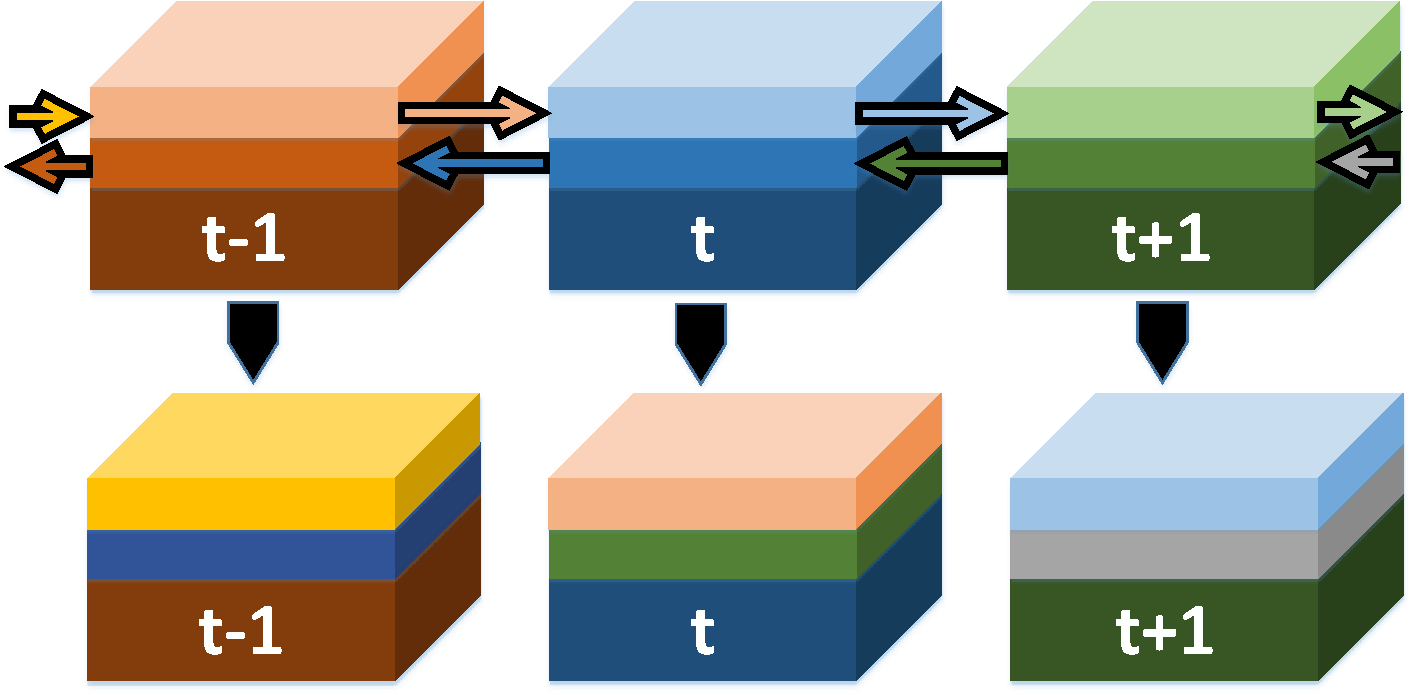
\includegraphics[width=0.7\textwidth]{Img/end/TSM_v1.pdf}
    \caption{时间聚合模块示意图。}
    \label{fig:TSM}
\end{figure}

\textbf{特征调制模块} 在获得模板特征 $f_{z}$ 和搜索图像的特征金字塔 $F_{x} = \{f_{x}^i\}_{i=1:5}$ 之后,对其进行调制以生成特定于目标的特征。
具体而言,使用全局平均池化操作根据 $f_{z}$ 生成调制矢量 $f_{avg}$,该调制矢量携带目标特定的表观信息。
%The search feature pyramid is $F = \{f_1, f_2, f_3\}$. 
%For $f_{x}^{i} \in F_{x}$, t
调制后的特征金字塔 $F_{mod} = \{f_{mod}^i\}_{i=1:5}$ 的生成方式如下:
\begin{equation}
    f_{mod}^i = \mathcal{M}(f_{avg}, f^i_x),
\end{equation}
其中 $\mathcal M(\cdot)$ 是逐通道互相关操作 \cite{SiamRPN++}。
%So we get the modulated feature pyramid $F_{mod} = \{f_{mod}^i\}_{i=1:5}$. 
%Then we predict proposals on $F_{mod}$.
每个调制后的特征图都被送入两个并行的全连接层中——通道尺寸为 $4k$ 的边框回归层和通道尺寸为 $2k$ 的边框分类层,其中 $k$ 是每个空间位置的最大候选目标数量。
% anchor 这个概念是必备的,所以是得讲一下。
%相对于一组锚定义了目标/背景标准和边界框回归。
我们根据 \cite{lin2017feature} 将具有相同尺度的锚框分配给每个不同的金字塔层级。有关锚框设置的详细信息,请参阅 \cite{lin2017feature}。
% For every modulated layer, we attach a classification layer and a regression layer to make predict.
\iffalse
The loss function of stage 1 is:
\begin{equation}
    \mathcal{L}_1 = 
\end{equation}
\fi
% you need to say how we get the candidates. Faster R-CNN already says it.
%The generated proposes with top-K classification scores is send to stage2.
我们使用得分最高的前 $N$ 个候选目标区域送入细化阶段进行后处理。

\subsection{对抗性 Dropout 模块}
%stage 1 的网络结构已经交代清楚了,就是一个FPN。和调制,和分类/回归层。那么stage的网络结构也应该交代清楚:roi align + 特征融合 + 对抗 + 分类/回归层。
\label{sec:stage2}
% 首先你要讲一下stage2在全局中的作用。
细化阶段旨在从候选目标区域中选择目标。
% 或许该讲一下stage2的输入包括:真实目标特征+候选区域。
% The input of stage 2 consists of: (1) The target feature is $f_{z} \in \mathbb R ^{256 \times 7 \times 7}$. (2) The candidate boxes generated from stage 1.
% Stage 2 compose of a feature merge module, a adversarial Dropout module, a classifier layer $h^{cls}$ and a regression layer $h^{reg}$. 
这些候选目标的特征使用 RoIAlign \cite{he2017mask} 操作从搜索特征金字塔 $F_{x}$ 中裁剪出来,然后与目标特征 $f_{z}$ 进行融合:
\begin{equation}
    \mathcal{X} = \mathcal{R}(b, F_{x}) \odot f_{z},
\end{equation}
其中 $\mathcal{R}$ 表示 RoIAlign 操作,$\odot$表示逐元素相乘操作,$b$表示候选目标区域,$\mathcal{X}$ 表示候选目标区域 $b$ 的融合特征。
%where $x' \in \mathbb R ^{256 \times 7 \times 7}$.
%$x' \in \mathbb R ^{256 \times 7 \times 7}$ is the feature of an RoI cropped from unmodulated feature pyramid using RoIAlign \cite{he2017mask}.
%The merged feature of a candidate target is:$x = x' \odot x_0$, where $\odot$ represents the element-wise multiplication. $x$ is the merged feature of that RoI.
% Maybe you need to say why you do the merge again.
% The modulation in stage 1 and the feature merge in stage 2 play different part in the tracking process. The modulation aims to detect the similar appearance in the whole image. The

\textbf{对抗性 Dropout} 特征融合之后,我们使用对抗性 Dropout \cite{park2018adversarial, lee2019drop} 来提高 $\mathcal{X}$ 的判别能力。
之所以使用这一模块,是因为 Dropout 是一种简单而有效的正则化方法,可以在训练过程中随机丢弃一部分神经元。Srivastava 等人 \cite{srivastava2014dropout} 指出, Dropout 具有整合网络的多个子集的作用。 Park 等人 \cite{park2016analysis} 着重指出了卷积层上的 Dropout 效果。Tompson 等人 \cite{tompson2015efficient} 指出,卷积层的激活通常被同一特征图中的类似激活所包围;因此,丢弃单个神经元在卷积层中没有强大的作用。取而代之的是,他们提出了空间 Dropout 的方法,即丢弃整个特征图,而不是单个神经元。 Hou 等人 \cite{hou2019weighted} 在空间 Dropout 的基础上,提出了一种加权的通道 Dropout 方案,该方案对各个通道使用可变的丢弃率,其中丢弃率取决于通道的平均激活值。加权通道 Dropout 仅应用于网络的较深层,在这些较深的层中,激活具有很高的特异性。
对抗性 Dropout 是一种用于监督和半监督学习的有效正则化方法。具体来说,Park 等人 \cite{park2018adversarial} 定义了两种类型的对抗性 Dropout:监督对抗性 Dropout(SAdD)和虚拟对抗性 Dropout(VAdD)。如果存在真实标注信息,可以使用 SAdD 最大化模型预测与真实标注信息之间的差异。另一方面,如果没有标签,则使用 VAdD 最大化输入的两个独立预测之间的差异。% Drop to Adapt: Learning Discriminative Features for Unsupervised Domain Adaptation
在本章种,我们引入对抗性 Dropout 以提高被跟踪目标的特征判别行。我们首先根据散度最大化预测对抗性 Dropout 掩码。将该掩码应用于 $\mathcal{X}$,以获得对抗性 Dropout 的特征。
然后,我们旨在最大程度地减少随机 Dropout 的特征和对抗性 Dropout 的特征之间的差异。
具体而言,令 $h^{cls}$ 和 $h^{reg}$ 分别表示细化阶段中的分类层和回归层。
根据 \cite{lee2019drop},按如下方式计算对抗性 Dropout 掩码:
\begin{equation}
\begin{split}
    & \mathbf{m}^{adv} = \mathop{\arg\max}\limits_{\mathbf{m}}D[h^{cls}(\mathcal{X} \odot \mathbf{m}^s), h^{cls}(\mathcal{X} \odot \mathbf{m})] \\
    & where~||\mathbf{m}^s - \mathbf{m}|| \leq \delta_e L,
\end{split}
\end{equation}
其中 $L$ 代表 $\mathbf{m} \in \mathbb R^L$ 的尺寸,
$\mathbf{m}^s$ 表示随机 Dropout 掩码, $\mathbf{m}^{adv}$ 表示对抗性 Dropout 掩码。
$\delta_{e}$ 是一个超参数,用于控制相对于 $\mathbf{m}^{s}$ \cite{lee2019drop} 的扰动幅度。
%and $\delta_{e}$ is a hyper parameter to control the perturbation magnitude with respect to $m^{s}$ \cite{lee2019drop}
$D[p, p'] \geq 0$ 测量两个分布 $p$ 和 $p'$ 之间的差异。

为了计算 $\mathbf{m}^{adv}$,\cite{park2018adversarial} 通过在计算过程中进行适当放松来优化 0/1 背包问题。有关详细信息,请参考 \cite{park2018adversarial}。
%Then, we use the mask to Dropout the feature, then send it to the classifier.
%We also send the clean feature to the classifier, and wish the loss minimum:
在生成 $\mathbf{m}^{adv}$ 之后,我们的目标是使关于 $\mathcal{X}$ 的两个预测分布之间的差异最小化:一个采用随机 Dropout 掩码 $\mathbf{m}^{s}$ 获得,另一个采用对抗性 Dropout 掩码 $\mathbf{m}^{adv}$ 获得 \cite{lee2019drop}。
\begin{equation}
    \mathcal{L}_{adv} = \mathbb E[D_{KL}[h^{cls}(\mathcal{X} \odot\mathbf{m}^{s})||h^{cls}(\mathcal{X} \odot\mathbf{m}^{adv}))]],
\end{equation}
其中 $D_{KL}$ 是 Kullback-Leibler 散度。

最后,对于每个候选目标区域,分类层在两个类别(前景或背景)上生成 softmax 概率估计,而回归层为前景类别输出四个实数值,用于编码候选目标区域的精确边界框位置。
SiamTFA 的损失是:
%The RoI Aligned features are fed into the global average pooling layer followed by two sibling output layers: one that produces softmax probability estimates over two classes (foreground or background) and another layer that outputs four real-valued numbers for the foreground class. These four values encode the refined bounding-box position for the RoI.
%We get the final tracking result as follows: The classification layer $h^{cls}$ predicts a score for a RoI, the regression layer $h^{reg}$ has shape * and predicts a 4-d vector for it.
%The RoI with the top score is the final box.
\begin{equation}
\mathcal{L} = \mathcal{L}_{cls}^{stage1} + \mathcal{L}_{cls}^{stage2} + \mathcal{L}_{reg}^{stage1}+\mathcal{L}_{reg}^{stage2} +  \lambda \mathcal{L}_{adv},
\end{equation}
其中 $\lambda$ 是用于平衡对抗损失和分类/回归损失的超参数。$\mathcal{L}_{cls}^{\cdot}$ 是交叉熵损失,$\mathcal{L}_{reg}^{\cdot}$ 是回归分支的平滑 $L1$ 损失。在测试过程中,具有最高分类得分的区域被选择为预测目标。


\iffalse
{classification/regression} The structure of $f^{cls}$ is ... The structure of $f^{reg}$ is ...
Suppose $B^*_t$ is the target bounding box at frame $t$, which is estimated through:
\begin{equation}
B^*_t = h^{reg}(\mathop{\arg\max}\limits_{x \in \mathcal{X}}h^{cls}(x)), 
\end{equation}
where $\mathcal{B}_t^1$ is a set of proposals generated from stage 1.
\fi

\section{实验评估与分析}

\begin{figure}[t]
    \centering
    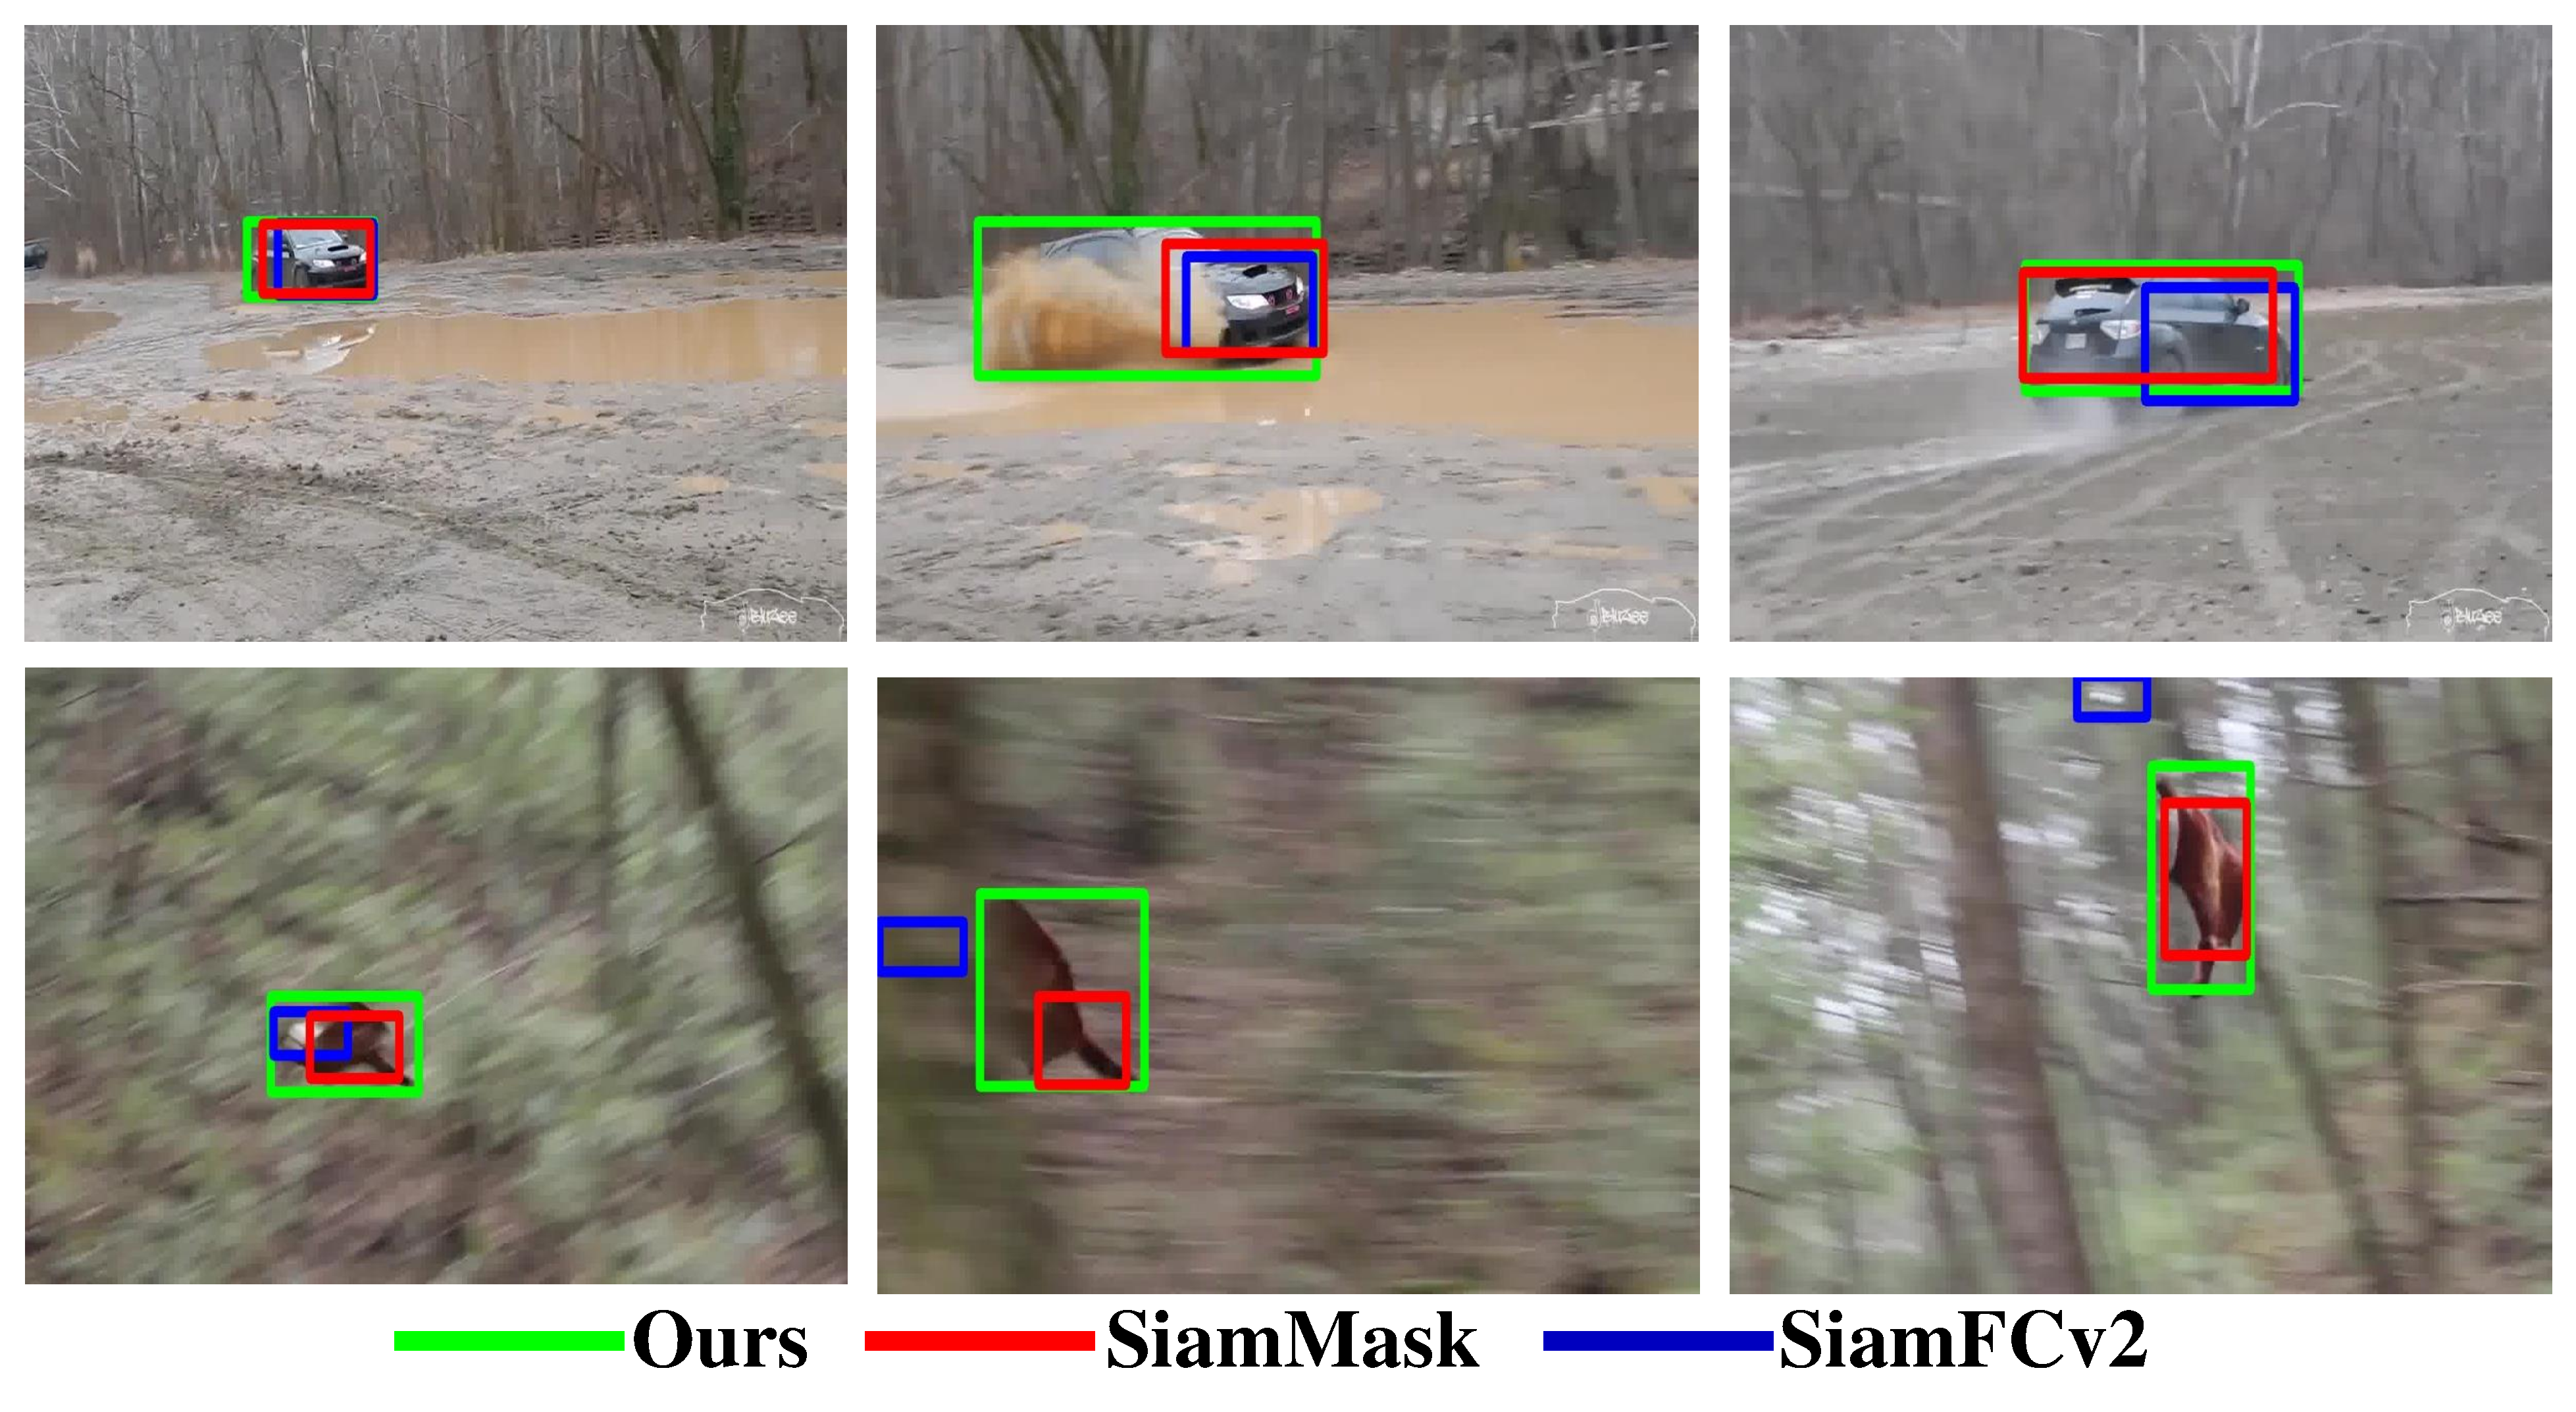
\includegraphics[width=1.0\textwidth]{Img/end/visulization.pdf}
    \caption{将我们的方法与 SiamMask 和 SiamFCv2 进行比较。示例框架来自 GOT-10k 测试装置。与现有方法相比,我们的方法可有效处理不良的目标表观。}
    \label{fig:visulization}
\end{figure}

在本节中,我们首先介绍实现细节。
然后,我们对 GOT-10K \cite{GOT-10k} 数据库和 UAV20L \cite{mueller2016benchmark} 数据数据库进行评估。
\subsection{实施细节}
本章提出的网络在 GOT-10k \cite{GOT-10k} 的训练集上进行训练,而骨干网络在 ImageNet 上进行了预训练。
我们应用动量​​为 0.9 的随机梯度下降,并将权重衰减设置为 0.0005。
学习率从 $10^{-2}$ 降至 $10^{-4}$。
批次大小设置为 2,并且对网络进行了 90000 次迭代训练。
我们的跟踪器是使用 PyTorch 在 Python 中实现的。
%First stage, we select 4000 proposals to send to stage2, the positive/negative rate is 1:3.
%To shift channels $K=2$.
%Because of the memory limit, the batch size is 2.
%To calculate the loss, $\lambda = 1$.
%For both training and testing, the size of a template image is 
% 其实有些对不上。按论文上讲,第一阶段是找到若干候选框。第二阶段是得到唯一结果。实际上是,第一阶段得到若干候选框,第二阶段进一步筛选得到约10个候选框(这才是真正的相似目标),然后按IoU和得分来选择最终结果。
% For test, we select top 100 proposals to send to stage2. The we use NMS to select top 10 object. 
\subsection{对 GOT-10k 数据集的评估}

\begin{figure}[t]
    \centering
    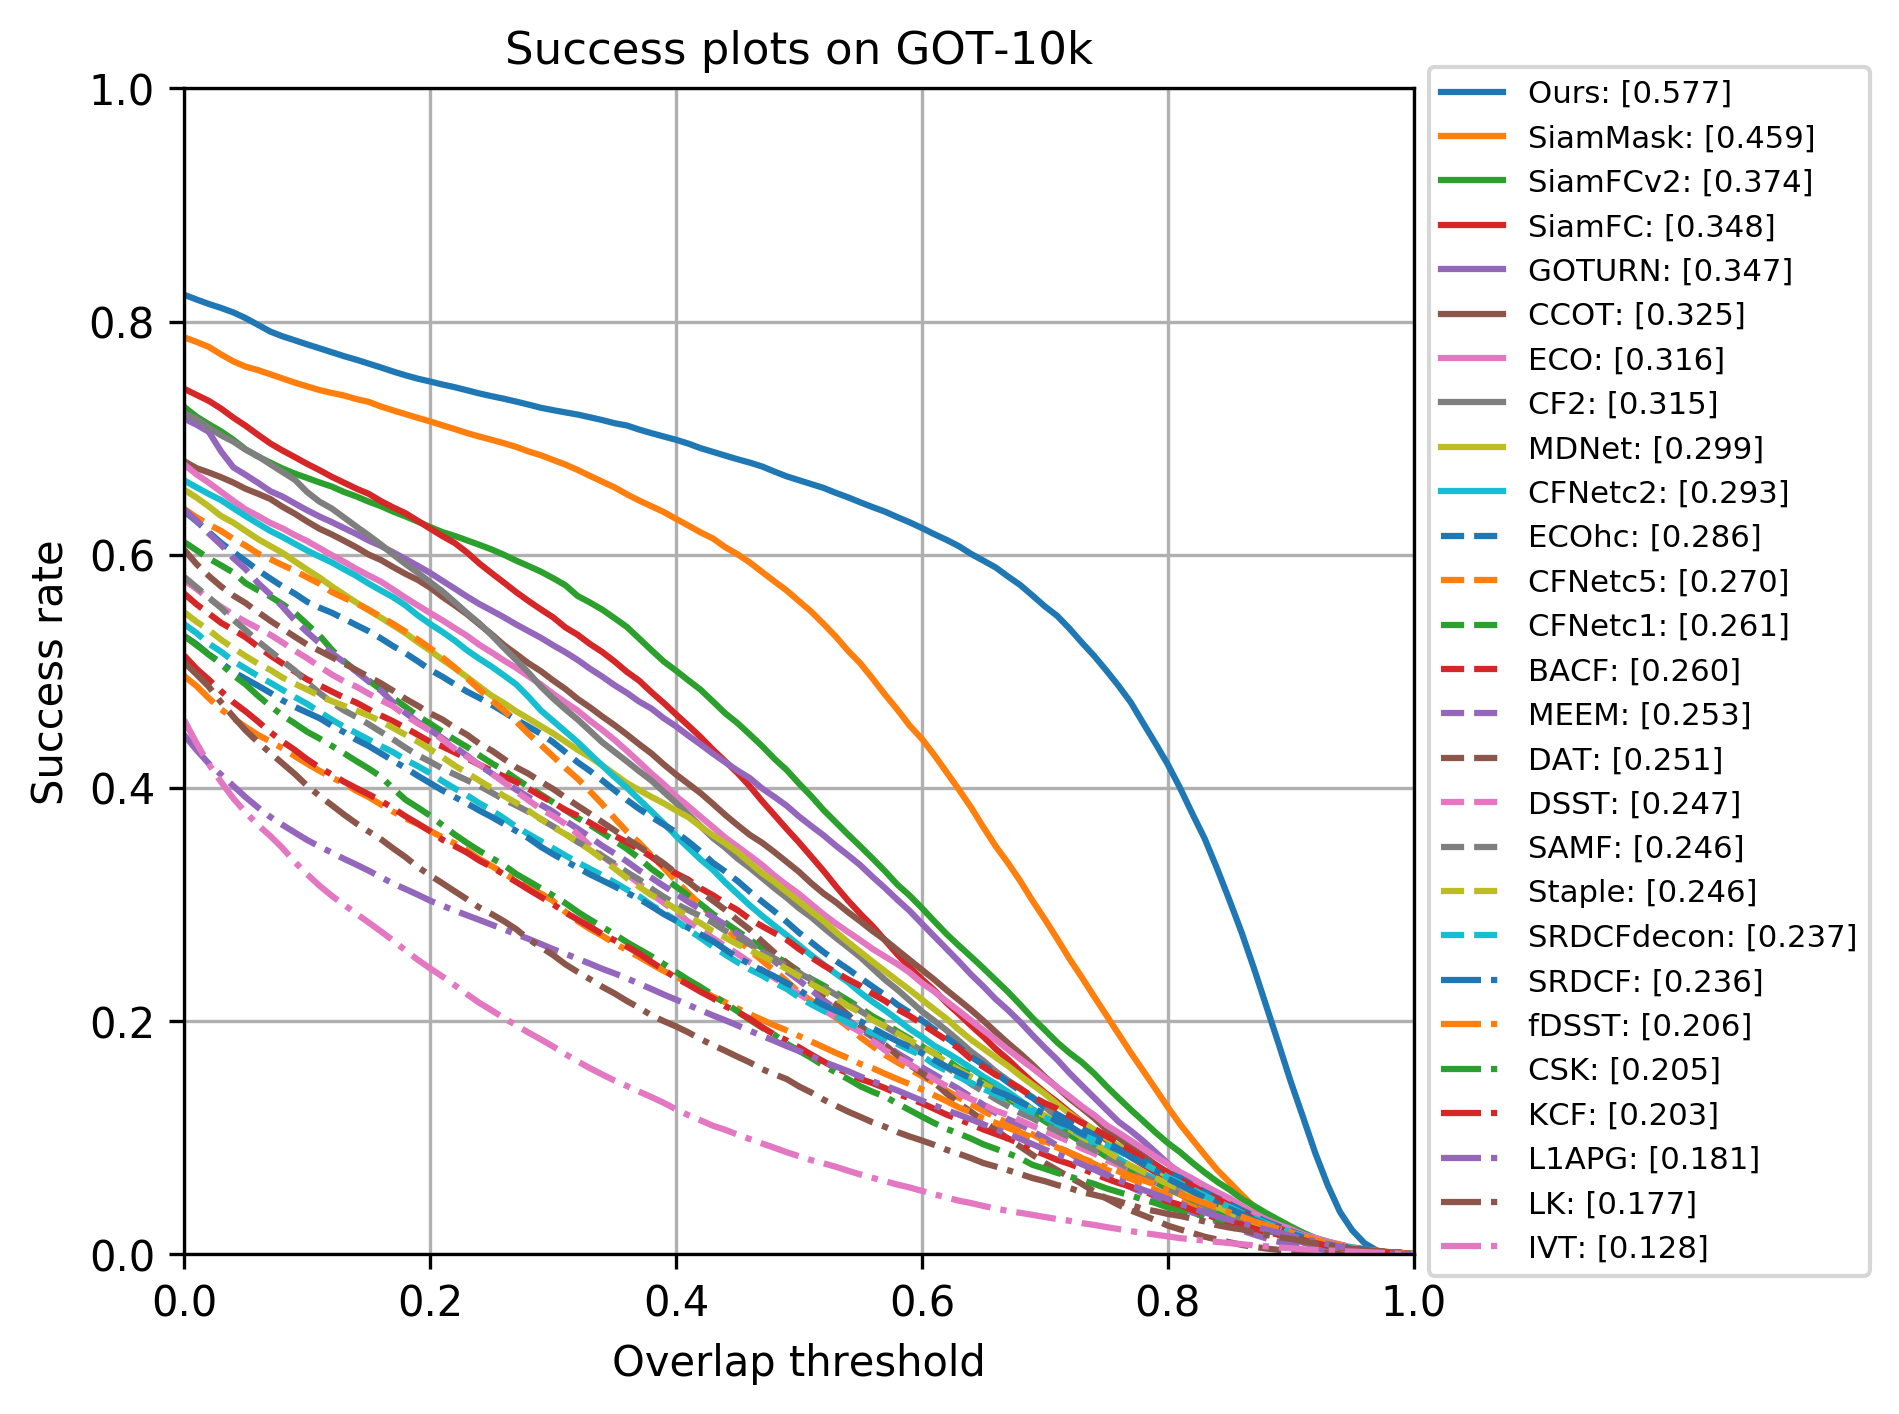
\includegraphics[width=1\textwidth]{Img/end/success_plot.png}
    \caption{GOT-10k 的总体性能,按其平均重叠(AO)得分进行排名。}
    \label{fig:got10k}
\end{figure}

\begin{table}[t]
\centering
\caption{我们的算法在 GOT-10k 测试集上具有不同组件的性能。}
\begin{tabular}{c c c c c}
\bottomrule
\begin{tabular}[x]{@{}c@{}}Temporal\\aggregation\end{tabular} & \begin{tabular}[x]{@{}c@{}}Adversarial\\Dropout\end{tabular} & $AO$ & $SR_{0.50}$ & $SR_{0.75}$ \\ 
\hline
          &           & 0.542 & 0.607 & 0.456 \\
\checkmark&           & 0.561 & 0.645 & 0.480 \\
\checkmark&\checkmark & 0.577 & 0.662 & 0.509 \\
\bottomrule
\label{tabel:ablation}
\end{tabular}
\end{table}

\begin{table}[t]
\centering
\caption{将我们的方法的结果与 GOT-10k 测试集上的其他方法进行比较。}
\begin{tabular}{l l l l}
\bottomrule
Method   &  $AO$   &  $SR_{0.50}$ & $SR_{0.75}$  \\
\hline
Ours &  $\textbf{0.577}^\textbf{1}$ & $\textbf{0.662}^\textbf{1}$  & $\textbf{0.509}^\textbf{1}$  \\
SiamMask &  0.459&  0.560 &0.205 \\
SiamFCv2 &  0.374&  0.404 &0.144 \\
SiamFC   &  0.348&  0.353 &0.098 \\
GOTURN	 &  0.347&  0.375 &0.124 \\
CCOT	 &  0.325&  0.328 &0.107 \\
ECO	     &  0.316&  0.309 &0.111 \\
CF2	     &  0.315&  0.297 &0.088 \\
MDNet	 &  0.299&  0.303 &0.099 \\
%CFNetc2	 &  0.293&  0.265 &0.087 \\
%ECOhc	 &  0.286&  0.276 &0.096 \\
\bottomrule
\end{tabular}
\label{table:got}
\end{table}
在本小节中,我们在 GOT-10k \cite{GOT-10k} 数据集上评估我们的方法。
% Say something about this dataset.
GOT-10k 是最近提出的目标跟踪数据集,包含 10000 多个视频序列,目标序列由轴对齐的边界框注释。
%Note that the classes between training and test sets are zero-overlapped. 
%This one-shot protocol avoids the evaluation bias towards familiar objects. 
GOT-10k 测试装置包括 180 种序列,具有 84 种不同的目标类别和 32 种运动模式。作为性能指标,我们使用 \cite{GOT-10k}中提出的平均重叠(AO)分数和成功率(SR)。AO表示所有地面和估计边界框之间重叠的平均值,而 SR 表示重叠超过 0.5/0.75 的成功跟踪帧的百分比。

\textbf{消融研究}
从表 \ref{tabel:ablation} (第 $1^{st}$ 行和第 $2^{nd}$ 行)中,我们看到,通过添加时间聚合模块,AO 性能提高了1.9%。
这是因为时间聚集模块通过聚集来自相邻帧的时间信息来改善每帧特征。
%The RPN stage rapidly filters out most background samples, and the RoI head adopts a fixed foreground-to-background ratio to maintain a manageable balance between foreground and background.
从表 \ref{tabel:ablation} (第 $2^{nd}$ 行和第 $3^{rd}$ 行)中,我们看到,通过对抗性 Dropout 模块,AO 增加了1.6%。
%This is because the proposed motion model can effectively predict the position distribution of the target, effectively avoiding the adverse effects of distractors. 
这是因为对抗性退出模块提高了我们的孪生跟踪网络的识别能力。

\textbf{总体效果}
我们将我们提出的方法与 8 个跟踪器(包括最新技术)进行了比较。
表 \ref{table:got}.
中显示了评估的跟踪器的性能。
与其他列出的方法相比,我们的方法实现了 0.577 的出色 AO。
ECO \cite{danelljan2017eco} 是基于 DCF 的最新跟踪器,它引入了分解卷积运算符,可显着减少 DCF 模型中的参数数量。 相比之下,我们的跟踪器基于强大的孪生架构。因此,我们的跟踪器的 AO 得分明显优于 ECO,提高了 26.1%,这表明孪生体系结构在目标跟踪任务方面的有效性。
SiamMask \cite{Wang2018SiamMask} 是最近提出的孪生跟踪器。它同时在三个任务上训练一个孪生网络,每个任务都对应一种不同的策略,以在新帧中建立目标目标和候选区域之间的对应关系。
但是,它是基于局部搜索机制的:在以上一帧的目标位置为中心的小邻域内搜索目标,且未充分利用时间信息。相比之下,我们的 SiamTFA 使用全局搜索机制。它始终能够感知整个图像上的目标,且能够充分利用时间信息。结果,我们的跟踪器在 AO 方面的性能优于 SiamMask 11.8%,这凸显了建议的时间聚合模块的重要性。

\begin{figure}[t]
\begin{minipage}[b]{0.5\textwidth}
  \centering
  \centerline{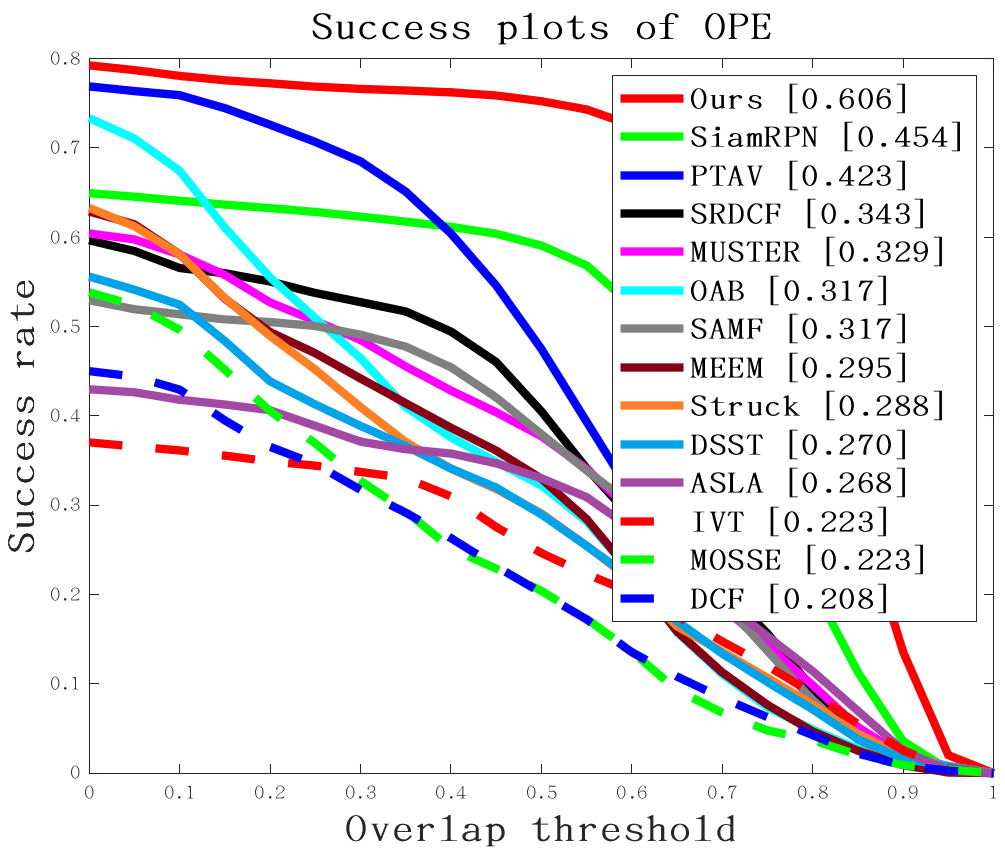
\includegraphics[width=1.0\textwidth]{Img/end/quality_plot_overlap_OPE_AUC.png}}
\end{minipage}
\hfill
\begin{minipage}[b]{0.5\textwidth}
  \centering
  \centerline{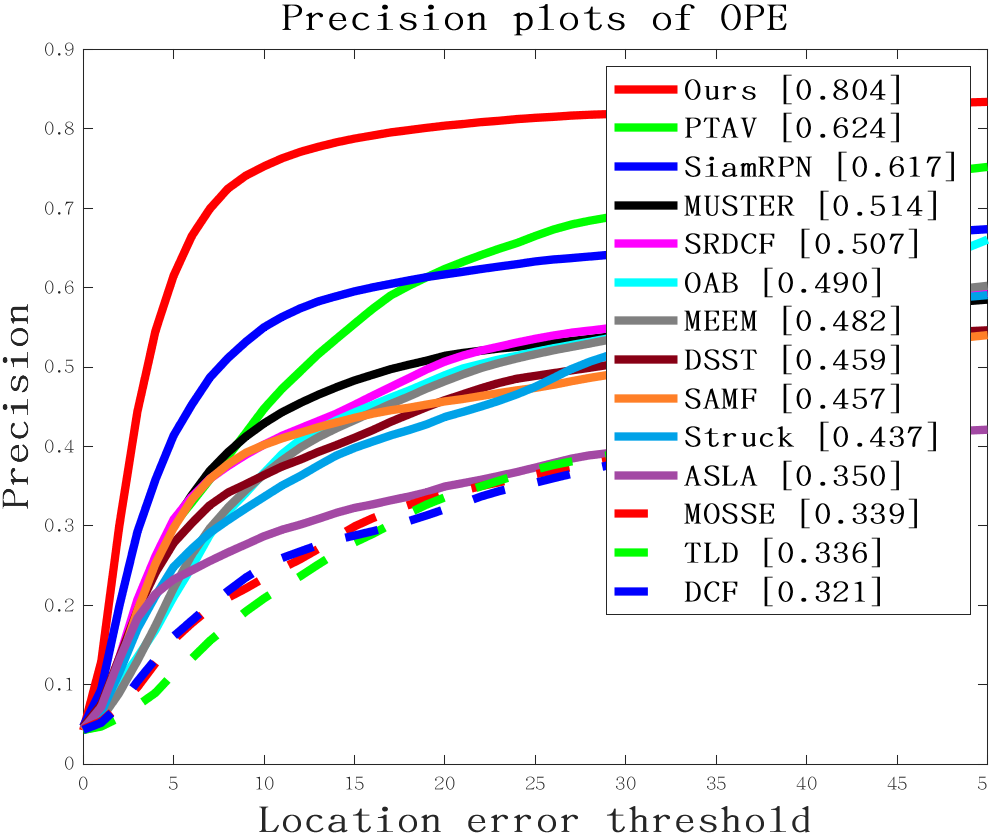
\includegraphics[width=1.0\textwidth]{Img/end/quality_plot_error_OPE_threshold.png}}
\end{minipage}
\caption{UAV20L 数据集上的成功图和精度图。}
\label{fig:uav20l}
\end{figure}
\subsection{对 UAV20L 数据集的评估}
在本小节中,我们在 UAV20L \cite{mueller2016benchmark} 长期跟踪数据集中评估跟踪器。
它包含从低空鸟瞰视角捕获的 20 个高清视频序列,平均序列长度为 2934 帧。
在此实验中,使用两种方法对所有跟踪器进行了比较:精度和成功率。精度的度量是预测边界框的中心与相应的地面真值边界框的中心之间的距离。成功是通过预测边界框内的像素与地面真实边界框内的像素并集的交点来衡量的。
在图 \ref{fig:uav20l} 中,我们可以发现,与某些代表性跟踪器相比,该算法具有更好的跟踪性能。
在成功图中,我们的跟踪器获得的 AUC 得分为 0.606。
在精度图中,所提算法的得分为 0.804。
它表明我们的跟踪器超越了其他最新算法,例如 SiamRPN \cite{SiamRPN} 和 PTAV \cite{fan2018parallel}。这证明了我们的跟踪器在长期跟踪情况下的有效性。

\section{结论}
在本章中,我们介绍了一种用于视觉目标跟踪的新型孪生架构。
具体来说,我们提出的算法包含两个主要模块,即时间聚合模块和对抗性删除模块。时间聚集模块通过聚集相邻帧的特征来改善每帧特征。对抗性 Dropout 模块提高了孪生跟踪网络的辨别能力。
大量的实验结果表明,所提出的算法的性能优于最新算法。